\chapter{Implementation} \label{implem}

This chapter describes the implementation of the methods for comparison of the performance in a disaster situation. The implementation is mainly focused on the comparison of accuracy of the models. A discussion on the implementation, including the humanitarian aspects, can be found in section \ref{sec:disc}.

\section{Preparation} \label{sec:prep}
\noindent In the preparation of this research various background information has been collected, the results of this research have been represented in chapter \ref{framework}. These results are based on literature studies and practical experience from the field regarding the use of damage data in the wake of a disaster. However, the methods selected for comparison have also been selected for their variety in data sources used. This guarantees the availability of either dataset in case of unseen disaster situations. To thoroughly compare the impact of data and methods, table \ref{tab:matr} has been developed for easier comparison. The goal of this matrix is the comparison between the influence of data and methods. Further more it allows for the exploration of comparable methods between datasets to achieve new methods and possibilities for classification. As the method by \citet{Yun2015} is developed for \ac{sar} data, a comparable method will need to be found or developed for optical data. Vice versa for the method described by \citet{Vetrivel2016b}, in this case the methods are written for optical data and should be considered for \ac{sar} data. Section \ref{sec:res} will elaborate on these comparable approaches to damage detection and how these might apply to damage classification. \\

\begin{table} [h]
	\centering
	\captionsetup{justification=raggedright,singlelinecheck=false}
	\caption{\footnotesize{Design matrix for combination of methods and data. Combinations have been abbreviated for continuity in text. These combinations are: \ac{eso}, \ac{ess}, \ac{cno}, and \ac{cns}.}}
	\begin{footnotesize}
		\begin{tabular}{m{2.5cm}|m{2.5cm}|m{2.5cm}|}
			\hline
			& Optical \ac{uav} Data & Satellite \ac{sar} Data \\ \hline
			Equalisation and subtraction & \ac{eso} & \ac{ess} \\ \hline
			Convolutional Neural Network & \ac{cno} & \ac{cns} \\ 
			\hline
		\end{tabular}
	\end{footnotesize}
	\label{tab:matr}
\end{table}

\section{Tools and datasets used} \label{tool}
Tools and data are necessary to facilitate the implementation of the methods in design matrix [Table \ref{tab:matr}]. the following sections provide a short overview of the tools and data used in the implementation. These relate to the methodology described in section \ref{sec:met} and methods selected in section \ref{sec:etech}.

\subsection{Tools}
The tools in table \ref{tab:tools} are select for the assessment of the existing methods as described in section \ref{sec:etech}. These are based on Open Source or Free to Use software packages as these are also available for deployment in the field by the \ac{nlrc}. Furthermore allow these package for more customisability for implementation with specific datasets. All code is available on GitHub \footnote{\url{https://github.com/DKersbergen/AutomatedDamageClassification}}. \\

\noindent Most of the implementation has been done using Python, this universal programming language is compatible with the other tools available for this research. Some steps required specialised algorithms, these steps are the following: [1.] To accommodate for the use of [visual] geo-programming, Qgis has been used. All code was written in Python but based on internal analysis methods from Qgis. Other geo-programming components have been done in Python using GDAL and OSR. [2.] For the specialised pre-processing and analysis performed on \ac{sar} imagery, the free to use \ac{esa} processing tool SNAP has been used. [3.] Lastly, to perform deep learning within the Python language, the module tflearn for Tensorflow has been used. This module has compatibility problems with Windows, therefore a \ac{wsl} has been used to accommodate this tool.
\begin{table} [H]
	\centering
	\captionsetup{justification=raggedright,singlelinecheck=false}	
	\caption{Tools and modules used in this research [Alphabetic order]}
	\begin{footnotesize}
		\begin{tabular}{lp{5cm}p{4cm}}
			\toprule
			Tool & Used for & Notes \\
			\midrule
			Python & General programming language, tflearn module available as implementation of Tensorflow & Most steps are done through automation via Python to ensure quick overviews of large datasets.\\
			Qgis & For visualisation, change detection, and Geo-referencing & -- \\
			SNAP & To prepare \ac{sar} datasets for change detection & Free to use [for non-profits] \ac{sar} processing software from \ac{esa}. \\
			Tensorflow & Machine learning tool, with pre-trained networks available & Used through a \ac{wsl} install of Ubuntu. \\
			\bottomrule
		\end{tabular}
	\end{footnotesize}
	\label{tab:tools}
\end{table}

\subsection{Data} \label{sec:data}
The data available for this research has been summarised in table \ref{tab:data}. These datasets have been guidance in the selection of methods to be implemented, as put forward in section \ref{sec:scope}.\\

\noindent The specifications of the datasets are provided in table \ref{tab:data}, including the sources. All datasets are available through the various portals. Ground truth data is excepted as it might contain sensitive data about the people on the island of St. Maarten. The portals for the data are [1.] OpenAerialMap \footnote{\url{www.openaerialmap.org}} for the \ac{uav} and aerial datasets, [2.] Copernicus Scihub \footnote{\url{scihub.copernicus.eu.org}} for the \ac{sar} datasets, [3.] the \ac{srtm} dataset has been acquired via a plug-in to the SNAP tool,  [4.] Turbo Overpass \footnote{\url{https://overpass-turbo.eu/}} has been used to acquire the building vector layer from OpenStreetMap \footnote{\url{www.openstreetmap.org}}, and [5.] lastly the \ac{stoa} data for damage classification from manual visual interpretation was retrieved from the Copernicus \ac{ems} Hub \footnote{\url{https://emergency.copernicus.eu/mapping/}}. Furthermore, it must be noted that not all UAV optical data is of the exact same resolution or from the exact date, therefore the average has been indicated in the table for the resolution and a interval for the dates. Lastly, the ground truth data is derived, by the 510 team of the \ac{nlrc}, from \ac{vhr} \ac{uav} imagery by visual interpretation following the principles discussed in section \ref{sec:clas}. Per dataset an example is provided.\\

\begin{table} [h]
	\centering
	\captionsetup{justification=raggedright,singlelinecheck=false}	
	\caption{Datasets with specifications, available for this research [Alphabetic order]}
	\begin{footnotesize}
		\begin{tabular}{lllp{2cm}ll}
			\toprule
			Platform & Technique & Resolution & Acquisition date & Source & fig.\\
			\midrule			
			Aerial & Optical & 0.2x0.2 m & 20-Feb-2017 & IGN  & \ref{fig:ign}  \\
			Satellite & \ac{sar} & 2.7x22 m & 11-Aug, 23-Aug, 16-Sept-2017 & Sentinel & \ref{fig:sar}   \\
			\ac{uav} & Optical & 0.04x0.04 m & 11-Sept-2017 -- 2-Oct-2017  & \ac{nlrc} -- RescUAV  & \ref{fig:uav}  \\
			Satellite & \ac{dem} & 30x30 m & unknown & \ac{srtm} & n/a \\			
			-- & Building outline & building & 2-Oct-2017 & OpenStreetMap & \ref{fig:build}\\
			-- & Ground truth & building & 2-Oct-2017 & \ac{nlrc} & \ref{fig:build}\\
			-- & \ac{stoa} & building & 14-Sept-2017 & Copernicus \ac{ems} & \ref{fig:build}\\
			\bottomrule
		\end{tabular}
	\end{footnotesize}
	\label{tab:data}
\end{table}
\begin{figure}[H]
	\centering
	\captionsetup{justification=raggedright,singlelinecheck=false}
	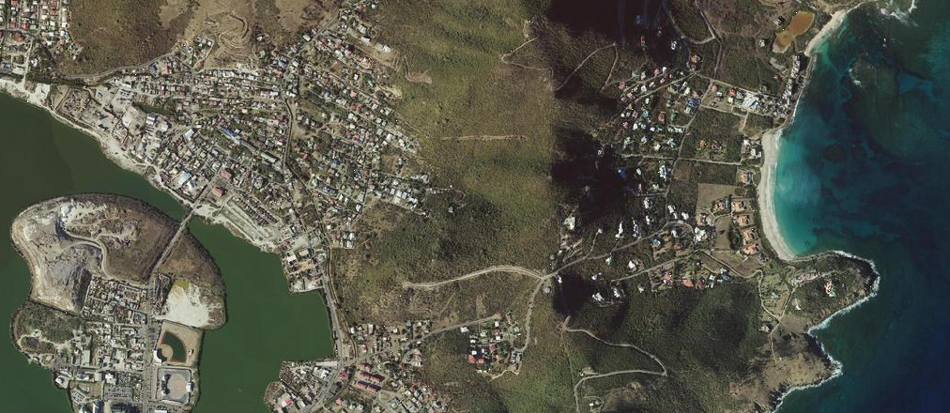
\includegraphics[width=0.95\textwidth]{figs/ign.png}
	\caption{\footnotesize{Example of aerial dataset [From: IGN France (16 Feb. 2017), Saint-Martin Orthoimage [georeferenced image], used under CC-BY4.0 as part of Open Imagery Network, retrieved from \url{www.openaerialmap.org}]}}
	\label{fig:ign}
\end{figure}
\begin{figure}[H]
	\centering
	\captionsetup{justification=raggedright,singlelinecheck=false}
	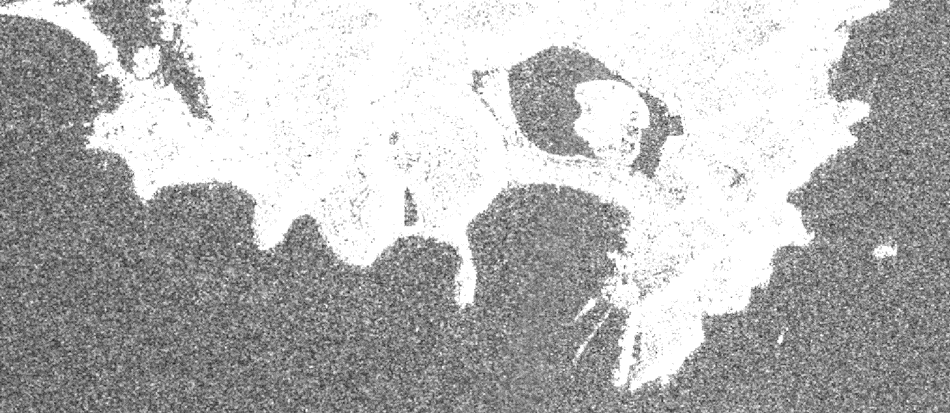
\includegraphics[width=0.95\textwidth]{figs/sar.png}
	\caption{\footnotesize{Example of \ac{sar} dataset [From: Copernicus Open Access Hub (2017), \ac{esa} [georeferenced image] - used under open access by In-Orbit Commissioning Review, retrieved from \url{scihub.copernicus.eu.org}]}}
	\label{fig:sar}
\end{figure}
\begin{figure}[H]
	\centering
	\captionsetup{justification=raggedright,singlelinecheck=false}
	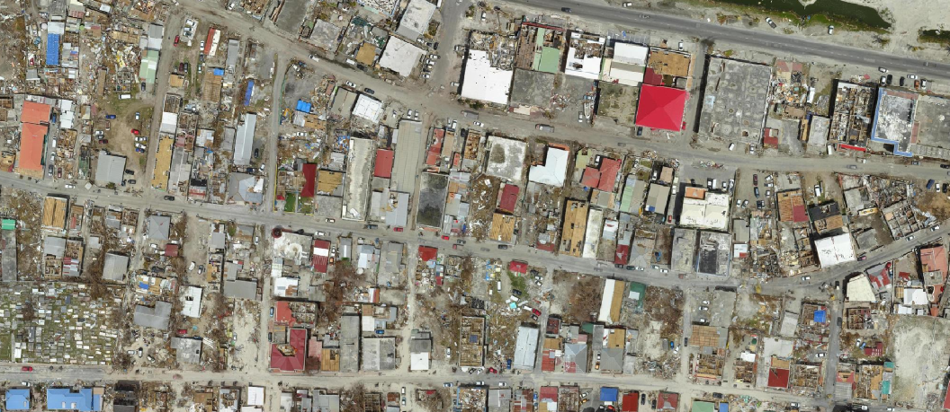
\includegraphics[width=0.95\textwidth]{figs/uav.png}
	\caption{\footnotesize{Example of \ac{uav} dataset [RescUAV (13 Sept. 2017), Philipsburg NE - Sint Maarten [georeferenced image], used under CC-BY4.0 as part of Open Imagery Network, retrieved from \url{www.openaerialmap.org}]}}
	\label{fig:uav}
\end{figure}
\begin{figure}[H]
	\centering
	\captionsetup{justification=raggedright,singlelinecheck=false}
	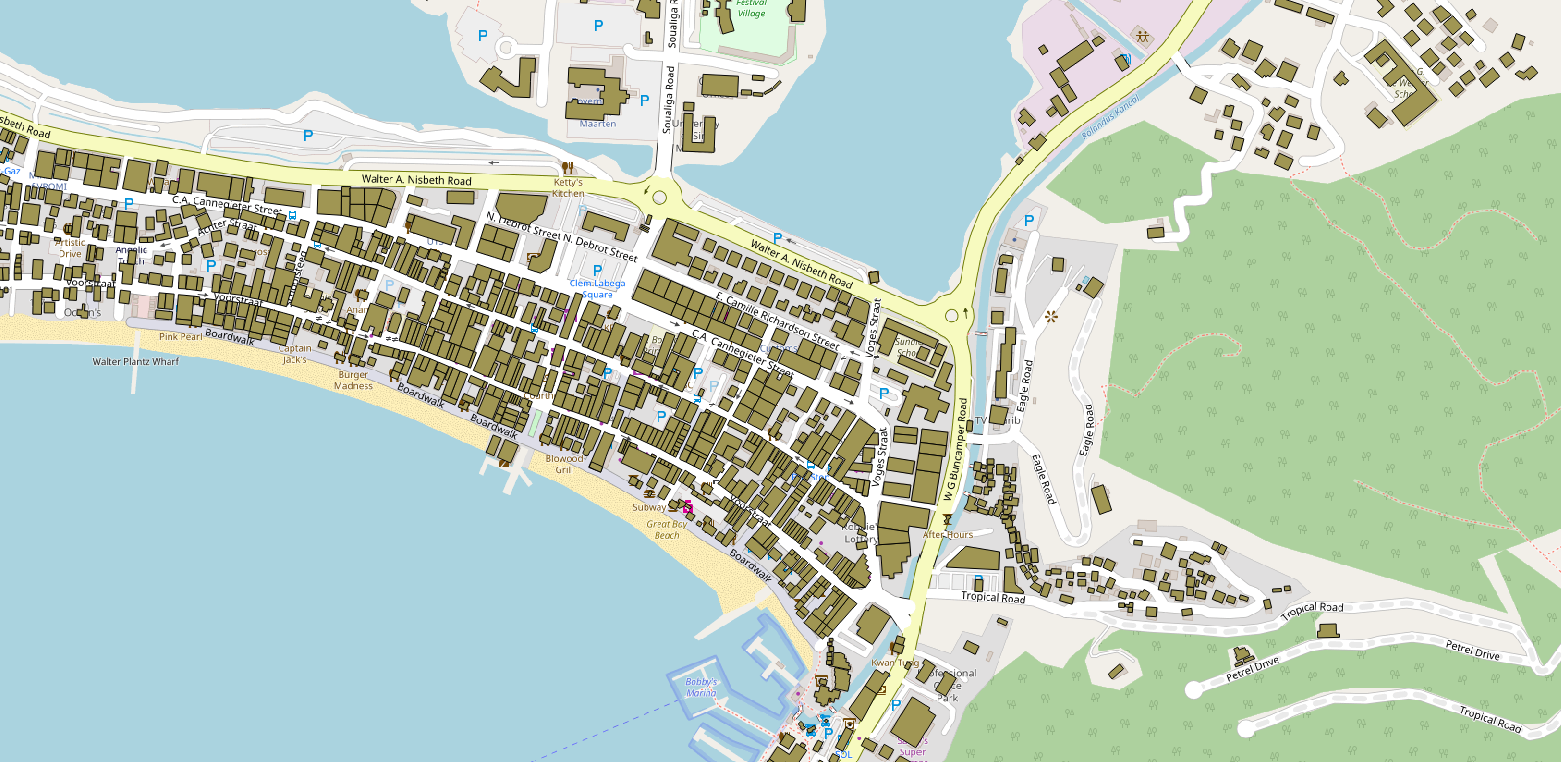
\includegraphics[width=0.95\textwidth]{figs/building.png}
	\caption{\footnotesize{Example of building dataset [From: OpenStreetMap contributors (2017), Philipsburg - Sint Maarten [georeferenced data], used under ODbL as part of OSMF, retrieved from \url{www.openstreetmap.org}]}}
	\label{fig:build}
\end{figure}
\section{Research implementation} \label{sec:res}
\noindent The research phase can be subdivided in the four subcategories described in table \ref{tab:matr}. This section will go into detail about the approach to each of these combinations of data and methodology, while the results will be presented in chapter \ref{result}.

\subsection{Equalisation and subtraction}\label{sec:Myun}
\subsubsection*{\ac{sar} data}
For the \ac{ess} approach, the method is already elaborated by \citet{Yun2015} and in section \ref{sec:yun}. This method has two clear phases, preprocessing and method implementation. Due to use restrictions, the software from \ac{nasa}, described by \citet{Yun2015}, is not available outside the United States and therefore this research. However, the \ac{esa} also provides similar tools in their SNAP package, which is available freely for use by \ac{ngo} as explained in section \ref{tool}. The methodology as described by \citet{Yun2015} can therefore still be implemented. The same steps will be followed for the pre-processing of the data, namely:

\begin{itemize}
	\item Set building through the pairing of the Sentinel 1 \ac{sar} datasets. These sets are labelled pre-event [11th of August 2016 paired with 23rd of August 2017] and post-event [23th of August 2016 paired with 16th of September 2017].
	\item Coherence mapping with a window of size 3 pixels in the azimuth direction, proportionally scaled to the \ac{sar} data available.
	\item Topographic phase removal using \ac{srtm} \ac{dem} data.
	\item Co registration of the various swaths using telemetry data.
	\item Terrain correction for geo-referenced result using  \ac{srtm} \ac{dem} data. \\
\end{itemize} 

\noindent The result of these steps are two coherence maps, pre-event and post-event respectively. In the combination of these coherence maps, the method determines if damage is present. To do this the histogram of the second coherence map is matched to the first, before univariate image differentiation is applied. This method is not described in detail by \citet{Yun2015}, so the following approach has been defined:

\begin{itemize}
	\item The array size of the post-event coherence map is determined
	\item Both coherence maps are flattened to a single list of pixels
	\item All unique pixels values are listed for both datasets 
	\item The cumulative distribution function is determined by normalising the cumulative sum of the amount of pixels in each map
	\item linear interpolation is used to match the statistics of the post-event map to that of the pre-event data\\
\end{itemize}

\noindent From here the matched coherence maps are subtracted from each other using univariate image differencing, in which each pixel value from the post-event coherence map is subtracted by the value of the pixel with the same X,Y coordinate in the pre-event coherence map [as described in section \ref{sec:yun}]. To visualise the change all change is considered absolute, in which an increase in pixel value can also be classified as change. Empirically a threshold will be set to determine the pixels classified as damage. As ground truth data is available this will be used to determine a more optimal threshold for the detection of damage. \citet{Yun2015} describe a masking technique which involved the human settlement index, this is used to focus the change detection on the areas in which people are living. However, as this research is focused on building scale level and building features available are, will this not be implemented and will the results be evaluated on a building scale.

\subsubsection*{Optical data} 
For the \ac{eso} approach similiar steps are implemented for the detection of damage using histogram matching and univariate image differencing. The optical data from \ac{uav}s differs from \ac{sar} data in various ways. First of all is the optical data available in products with 3 bands namely \ac{rgb}. Furthermore, only one dataset is available from before the disaster [aerial optical imagery from the IGN], as well as one after the disaster [\ac{uav} optical imagery from the \ac{nlrc} and RescUAV]. This requires a different approach the the pre-processing of the data before histogram matching and univariate image differencing can be implemented. To achieve a comparable approach, one band simplification of the dataset is applied. the optical imagery will be transformed to a \ac{hsv} image, of which each band is considered separate. Though this process the image is changed from a mix of colours to a description of features within the colour space, as described in section \ref{sec:relb}. In this new description of the data, three key characteristics of colour are described, particularly the Hue of a pixel, the Saturation, and the Value. For change detection it is important to understand what feature changes in case of damage. As can be seen in figures \ref{fig:colourchange} and \ref{fig:hsv} the saturation of an object describes the presence of colour. This clearly does shift in the case of damage sustained to a building. From the same figures, the hue of a building might change not as much, as the colours are roughly the same or of the same family in the pre-event and post-event imagery. Lastly the value, this seem to change quiet a bit during a disaster in which the amount of light reflected from a building clearly decreases as more light is bounced around between the rouble before it is bounced back, hence a decrease in lightness. For this method comparison all three reductions of information however are considered and taken into account in chapter \ref{implem}. Considerations with all of the simplifications, from \ac{rgb} to single \ac{hsv} layers, concern the time shift between images, creating other artefacts or noise. An example of this is the value change due to a different lighting condition. However the histogram matching as used by \citet{Yun2015} does account for these changes in lighting, reducing the amount of artefacts or false positives. \\

\begin{figure}[!h]
	\centering
	\begin{subfigure}{.475\textwidth}
		\centering
		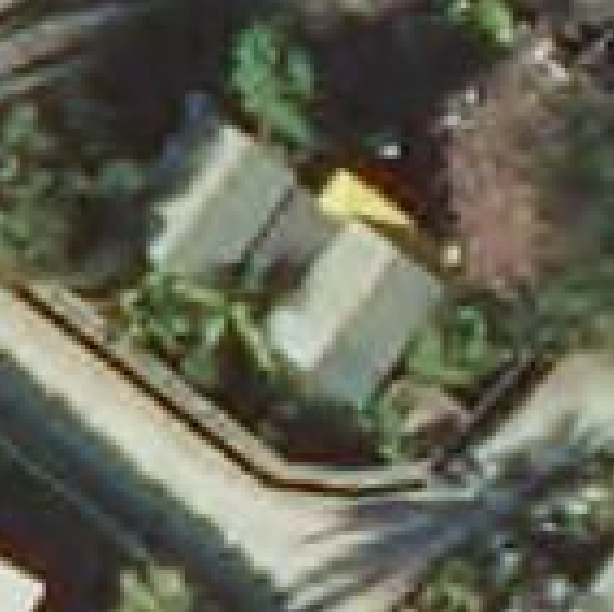
\includegraphics[width=.85\linewidth]{figs/CohB.png}
		\caption{\footnotesize{Colour representation of image pre-event}}
	\end{subfigure}
	\begin{subfigure}{.475\textwidth}
		\centering
		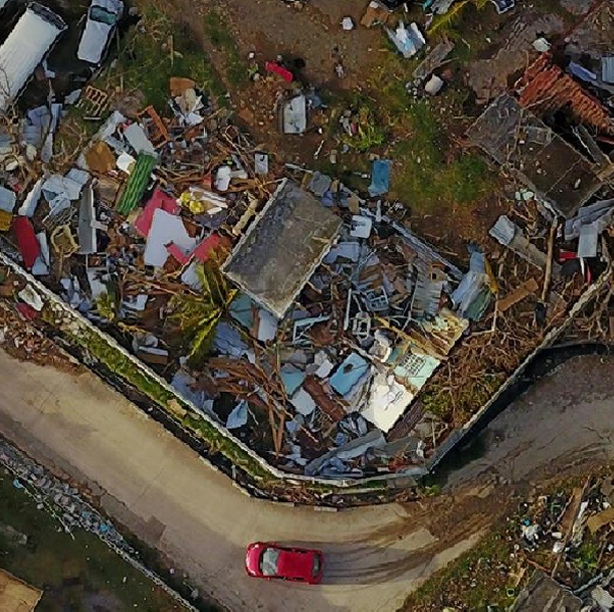
\includegraphics[width=.85\linewidth]{figs/CohA.png}
		\caption{\footnotesize{Colour representation of image post-event}}
	\end{subfigure}
	\caption{\footnotesize{Change between pre-event and post-event colour. Structure within an image. [From: a: IGN France (16 Feb. 2017), Saint-Martin Orthoimage [georeferenced image] | b: Netherlands Red Cross (15 Sept. 2017), Quilletor Dr - Sint Maarten [georeferenced image] | both used under CC-BY4.0 as part of Open Imagery Network, retrieved from \url{www.openaerialmap.org}]}}
	\label{fig:colourchange}
\end{figure}

\noindent The reduction from a three layered \ac{rgb} dataset to a single layered map of the data allows for the implementation of histogram matching as described for the \ac{sar} data in the previous subsection. However, as the pre-event and post-event datasets are not of the same resolution [table \ref{tab:data}] an extra step of pre-processing is necessary before the univariate image differencing can be used. In this step the post-event image will be down-sampled using the algorithm defined by Lanzcos [represented by equations: \ref{eq:lanczos}], as it performs best along other re-sampling algorithms \citep{Narendra2013}. From here an empirically set threshold can be used to determine the damage detection, which can be combined with an informed approach by optimising the threshold using ground truth data.

\begin{equation}
L(x) = 
\begin{cases} 
sinc(x).sinc(X/a) & \text{if} -a < x < a\\
0 & \text{elsewhere}
\end{cases}
\label{eq:lanczos}
\end{equation}

\subsubsection*{Classification}
To extent the method described by \citet{Yun2015}, to allow for classification, an empirically set thresholds can be used to determine more classes than only detection. However, this is only possible if the groups of damaged features are clearly distinguishable in the datasets acquired. This does not translate to a clear identification by visual interpretation, but clear distribution along the pixels classified for change, with correct density functions. A clear density function can allow for the identification of the damage classes, as described by \citet{Theodoridis2009} [figure \ref{fig:pdf}]. Aided by the existing ground truth data on building level, the threshold will be set empirically to determine the correct classification for damage.

\begin{figure}[!h]
	\centering
	\captionsetup{justification=raggedright,singlelinecheck=false}
	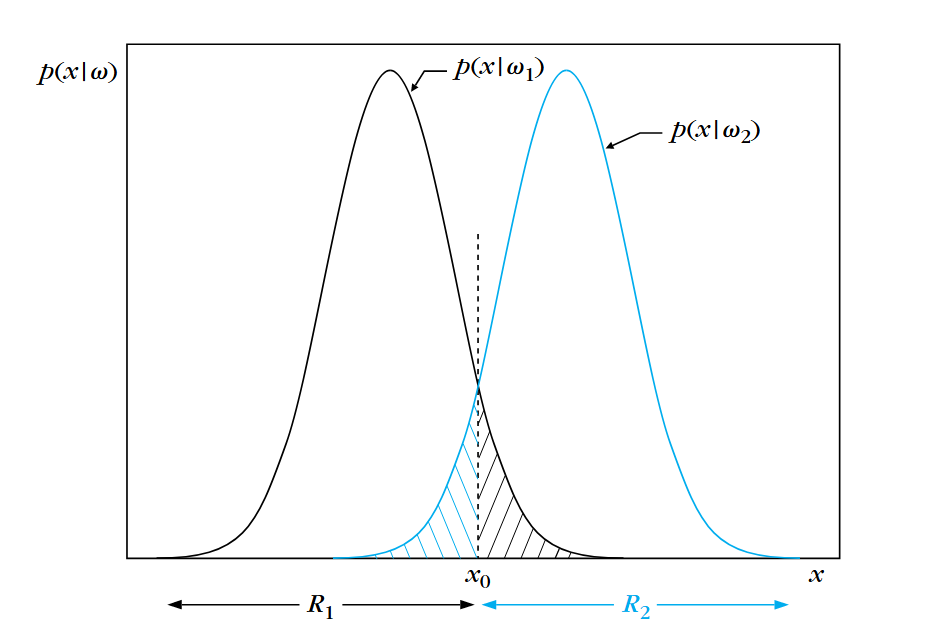
\includegraphics[width=0.95\textwidth]{figs/pdf.png}
	\caption{\footnotesize{Probability density function used for object classification with two classes [From: \cite{Theodoridis2009}}]}
	\label{fig:pdf}
\end{figure}

\subsection{Convolutional Neural Network} \label{sec:Mvet}
\subsubsection*{Optical data} 
For the \ac{cno} approach, the method described by \citet{Vetrivel2016b} is applicable. The steps remain relatively similar for this research, however as this is a comparison the \ac{cnn} defined in the paper has been used. To detect damage on the optical dataset using \ac{cnn}, the following steps will be taken.
\begin{itemize}
	\item Feature creation
	\item Neural network training
	\item Classification of samples\\
\end{itemize} 

\noindent Due to the availability of features from OpenStreetMap, the feature creation step will vary from the approach by \citet{Vetrivel2016b}. In this research a bounding box around the objects will be determined, based on the outline of the buildings acquired from OpenStreetMap via the Missing Maps \footnote{\url{www.missingmaps.org}} initiative. For a neural network, inputs with the same dimensions are beneficial. To ensure all features are of the same size and dimensions, the bounding boxes are taken as squares around the building features. These bounding boxes are used to cut features from the post-event \ac{uav} optical imagery. The resulting features are then rescaled to be the same pixel dimensions, namely 100 x 100 pixels. These are introduced to the Neural Network as described in figure \ref{fig:vet1}. 70\% of this dataset is used for training the \ac{cnn}, while the other 30 \% is used as validations set, this to the parameters described by \citet{Vetrivel2016b}. The learning rate is set to 0.001 to allow for swift learning while ensuring no over-fitting occurs due to a large learning rate. The resulting trained network is saved and used as input for the classification of an unseen dataset. This unseen dataset is a set of features extracted from the main set before training. Geographically this set is defined by the area described in chapter \ref{result}. This set will be used in the results phase for comparison. 

\subsubsection*{\ac{sar} data}
In the \ac{cns} approach, the same definition as for the \ac{cno} approach can be used with regards to the use of a \ac{cnn} for damage detection. In this approach, the features can be created from the post-event \ac{sar} data in the pre-processing phase, in contrast to the post-event \ac{uav} data described in the previous subsection. However, the data used in this research is not compatible with such approach as will be elaborated upon in chapter \ref{implem}.

\subsubsection*{Classification}
\ac{cnn} methods are very suitable for extension of the classification classes, in this case from two to four. A network can be trained for four classes instead of two by simply tweaking the deeper layers of the network. However, as networks are usually designed for a specific goal there is no guarantee that \ac{cnn} architectures available for damage detection will also work for damage classification with multiple classes. For this research the same network will be re-trained for the classification of the images to 4 classes. In this approach the same features will be used, however the training and validation set will be classified differently. This diversification of the dataset results in a decline of features per class, which can negatively impact the performance of the method.

\section{Assessment of Results} \label{sec:resu}
\noindent To allow for a good comparison between the ground truth data, methods described in this chapter, and visual interpretation as used by Copernicus \ac{ems}, various techniques for the rating of inter-rater agreement will be used. These will be the Cohen Kappa Score, the resulting confusion matrices, and the F1 score. All of these methods are used to determine the consensus between the prediction and ground truth data, as described in section \ref{sec:interrater}. Furthermore, will these principles also be used for the performance rating of the various empirically set thresholds for the method described by \cite{Yun2015}. The guiding principle in the selection of results will be the Cohen Kappa Score. Agreement is seen as good within this context and is therefore used for interpretation of the methods.

